\usetikzlibrary{arrows}
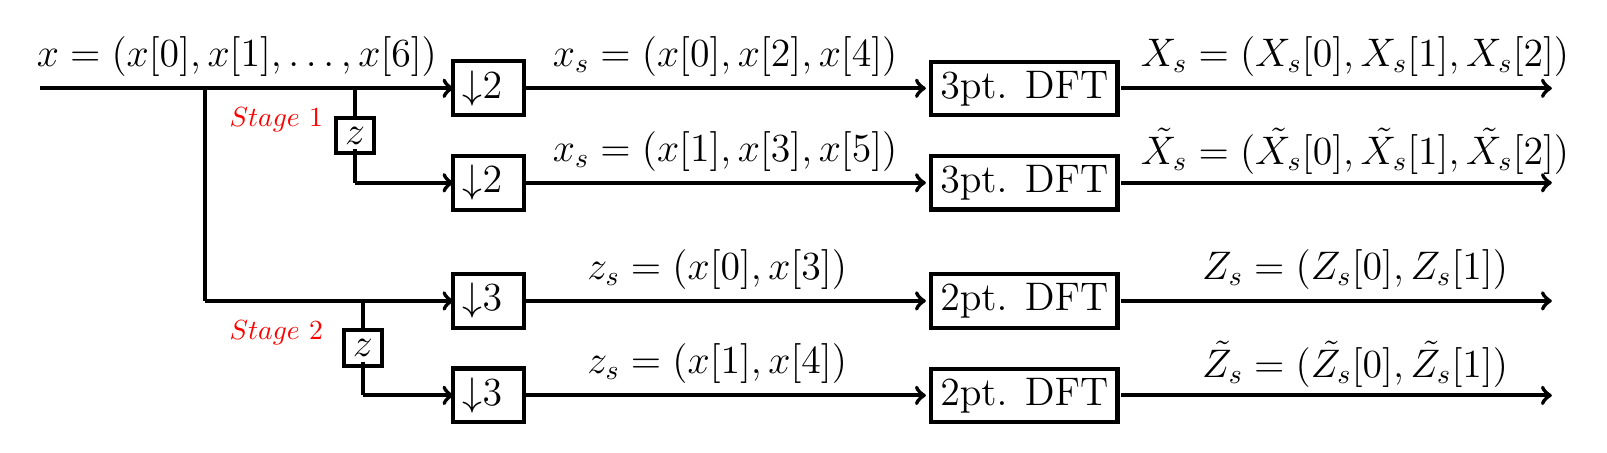
\begin{tikzpicture}

 % Downsampling blocks
\node[draw,align=center,thick,line  width =1.5pt] at (1.6,5.2) { \Large{$\mathbf{\downarrow} 3$} };
\node[draw,align=center,thick,line  width =1.5pt] at (1.6,6.4) { \Large{$\mathbf{\downarrow} 3$ }};

\node[draw,align=center,thick,line  width =1.5pt] at (1.6,7.9) {\Large{$\mathbf{\downarrow} 2$} };
\node[draw,align=center,thick,line  width =1.5pt] at (1.6,9.1) {\Large{$\mathbf{\downarrow} 2$ }};

%  Input lines to the down-sampling block
 \draw[->,thick,line  width =1.5pt] (0,5.2) -- (1.15,5.2);
 \draw[->,thick,line  width =1.5pt] (0,6.4) -- (1.15,6.4);
  
 \draw[->,thick,line  width =1.5pt] (-0.1,7.9) -- (1.15,7.9);
 \draw[->,thick,line  width =1.5pt] (-0.1,9.1) -- (1.15,9.1);

%  Delay blocks
\node[draw,align=center,thick,line  width =1.5pt] at (0,5.8) {\Large{$z$}};
\node[draw,align=center,thick,line  width =1.5pt] at (-0.1,8.5) {\Large{$z$}};

% paths connecting the delay blocks
 \draw[thick,line  width =1.5pt] (0,5.2) -- (0,5.63);
 \draw[thick,line  width =1.5pt] (0,6) -- (0,6.4);
 
 \draw[thick,line  width =1.5pt] (-0.1,7.9) -- (-0.1,8.33);
 \draw[thick,line  width =1.5pt] (-0.1,8.7) -- (-0.1,9.1);
 
% paths connecting the two stages   
 \draw[thick,line  width =1.5pt] (-0.1,9.1) -- (-2,9.1);
 \draw[thick,line  width =1.5pt] (0,6.4) -- (-2,6.4);
 \draw[thick,line  width =1.5pt] (-2,6.4) -- (-2,9.1);
  \draw[thick,line  width =1.5pt] (-4.1,9.1) -- (-2,9.1);
  
  
  
  % DFT blocks
\node[draw,align=center,thick,line  width =1.5pt] at (8.4,5.2) {\Large{2pt. DFT}};
\node[draw,align=center,thick,line  width =1.5pt] at (8.4,6.4) {\Large{2pt. DFT}};

\node[draw,align=center,thick,line  width =1.5pt] at (8.4,7.9) {\Large{3pt. DFT}};
\node[draw,align=center,thick,line  width =1.5pt] at (8.4,9.1) {\Large{3pt. DFT}};

% Connectors
 \draw[->,thick,line  width =1.5pt] (2.05,9.1) -- (7.15,9.1);
 \draw[->,thick,line  width =1.5pt] (2.05,7.9) -- (7.15,7.9);
  
 \draw[->,thick,line  width =1.5pt] (2.05,6.4) -- (7.15,6.4);
 \draw[->,thick,line  width =1.5pt] (2.05,5.2) -- (7.15,5.2);

 \draw[->,thick,line  width =1.5pt] (9.63,9.1) -- (15.1,9.1);
 \draw[->,thick,line  width =1.5pt] (9.63,7.9) -- (15.1,7.9);
 
 \draw[->,thick,line  width =1.5pt] (9.63,6.4) -- (15.1,6.4);
 \draw[->,thick,line  width =1.5pt] (9.63,5.2) -- (15.1,5.2);
 
 
  % Labels
  \node[draw=none,align=center,thick,line  width =1.5pt] at (-1.6,9.5) {\Large{$x=(x[0],x[1], \ldots, x[6])$}};
  
  \node[draw=none,align=center,thick,line  width =1.5pt] at (4.6,9.5) {\Large{$x_{s}=(x[0],x[2],x[4])$}};
  \node[draw=none,align=center,thick,line  width =1.5pt] at (4.6,8.3) {\Large{$x_{s}=(x[1],x[3],x[5])$}};
  \node[draw=none,align=center,thick,line  width =1.5pt] at (4.5,6.8) {\Large{$z_{s}=(x[0],x[3])$}};
  \node[draw=none,align=center,thick,line  width =1.5pt] at (4.5,5.6) {\Large{$z_{s}=(x[1],x[4])$}};
  
  \node[draw=none,align=center,thick,line  width =1.5pt] at (12.6,9.5) {\Large{$X_{s}=(X_{s}[0],X_{s}[1],X_{s}[2])$}};
  \node[draw=none,align=center,thick,line  width =1.5pt] at (12.6,8.3) {\Large{$\tilde{X_{s}}=(\tilde{X_{s}}[0],\tilde{X_{s}}[1],\tilde{X_{s}}[2])$}};
  \node[draw=none,align=center,thick,line  width =1.5pt] at (12.6,6.8) {\Large{$Z_{s}=(Z_{s}[0],Z_{s}[1])$}};
  \node[draw=none,align=center,thick,line  width =1.5pt] at (12.6,5.6) {\Large{$\tilde{Z_{s}}=(\tilde{Z_{s}}[0],\tilde{Z_{s}}[1])$}};
  
  
  
   \node[draw=none,align=center,thick,line  width =1.5pt] at (-1.1,8.7) {\color{red}$Stage ~1$};
  \node[draw=none,align=center,thick,line  width =1.5pt] at (-1.1,6) {\color{red}$Stage ~2$};
   
%\draw [thick](-2,4.6) --  --  ;
 
\end{tikzpicture}